%!TEX root = ./guide2seminars.tex
%!GEDIT texmaster = ./guide2seminars.tex
% mainfile: ./guide2seminars.tex
%
% Copyright © 2011 - 2020 DBIS Group, WWU Münster, in particular:
%           Till Haselmann <haselmann@wi.uni-muenster.de>
%           Florian Stahl  <flst@wi.uni-muenster.de>
% All rights reserved.
%

\section{Motivation}
Das Lernen mit Karteikarten gehört zu den beliebtesten Lernmethoden. Durch die Digitalisierung können die Lernenden die Karteikarten nun jederzeit und von überall aus lernen und so jede freie Zeit effizient nutzen. Voraussetzung hierfür ist eine geeignete Anwendung, die alle gewünschten und notwendigen Funktionen dazu bereitstellt. Weiterhin sind effektive Lernalgorithmen zur nachhaltigen Speicherung des Wissens in das Langzeitgedächtnis erforderlich. Die hier untersuchten Karteikarten-Anwendungen weisen sowohl bei den Funktionalitäten, wie auch bei den Lernalgorithmen oder dem Design diverse Mängel auf. Beispiele für diese Mängel sind unausgereifte Eingabemethoden für mathematische und chemische Formeln oder auch überladene und weniger motivierende Benutzeroberflächen. Weiterhin sollte Bildung, sowie auch Software zur Festigung und Erstellung von Bildungsmaterial für jeden frei zugänglich sein. Jedoch zeigt sich, dass viele der untersuchten Anwendungen kostenpflichtig sind.\\

Es gibt vielfältige Einsatzmöglichkeiten für die hier konzipierte Karteikarten Anwendung. Neben einer öffentlichen Bereitstellung kann die Anwendung auch für interne Einsätze, durch den Betrieb auf private Server verwendet werden. So können beispielsweise Universitäten, Schulen, Plattformen und Unternehmen ihren Studenten, Schülern, Kunden oder Mitarbeitern die Möglichkeit bieten ihr Wissen zu bestimmten Thematiken zu festigen. Für die Unternehmen hat dies den Vorteil von gebildeteren und besser geschulten Personal. Für Schulen und Universitäten kann dies ein höheres Ansehen durch fortschrittlichere Lernumgebungen ermöglichen und für Lernende hat dies eine Verbesserungen der Lernbedingung zur Folge. Da der Quellcode für jeden öffentlich zur Verfügung steht, ist der Einsatz auch mit keinerlei Kosten verbunden und dient hauptsächlich zur Förderung der Bildung und zur Festigung von Wissen in das Langzeitgedächtnis. 


Ziel dieser Seminararbeit ist die Entwicklung einer Applikation unter den Anforderungen von Open Educational Resources. Sie sollte ohne spezielle Fachkenntnis nutzbar sein, auch für diejenigen, die eine geringe Affinität zu Computern besitzen. Eine weitere Funktionsgruppe, die bei der Entwicklung berücksichtigt werden soll sind effiziente Lernalgorithmen und die Erstellung einer kollaborativen Plattform. In dieser Plattform sollen die Nutzer später in der Lage sein ihre Karteikarten mit anderen zu teilen und gemeinschaftlich daran zu arbeiten. Gerade im Rahmen eines Studiums kann eine kollaborative Erstellung von Materialien viel wertvolle Zeit sparen, sofern schon Material zur Verfügung steht. \\

Um dieses Ziel zu erreichen, werden zunächst verschiedene Anforderungen identifiziert. Im Sinne von Open Educational Resources werden technische Anforderungen, die in einem Selbstversuch von Dr. Jens Lechtenbörger aufgelistet wurden, verwendet \cite{Lechtenborger.2019}. Um ein effektives Lernen zu ermöglichen werden im einem nächsten Schritt verschiedene Lernalgorithmen erläutert. Im Anschluss zur weiteren Festlegung von Anforderungen werden noch eigene Erfahrungen mit einbezogen. Um die aktuelle Marktsituation auszuwerten, werden im nächsten Abschnitt verschiedene bekannte Karteikarten-Anwendungen evaluiert. Im letzen Kapitel dieser Seminararbeit wird das Konzept der Karteikarten-Anwendung Kicards vorgestellt, indem zunächst die gewünschten Funktionen nach Prioritäten aufgelistet werden. Nach Festlegung der Funktionen wird nachfolgend das Datenbankmodell modelliert und anschließend wichtige Funktionen erläutert. Zum Abschluss wird der aktuelle Entwicklungsstand und die weitere Vorgehensweise dargelegt, die über diese Seminararbeit hinausgehen.

\section{Anforderungen}
Für ein wohl überlegtes und ausgearbeitetes Konzept sind zunächst wichtige Anforderungen an einer Karteikarten-Anwendung erforderlich. Hierzu werden zunächst technische und allgemeine Kriterien aus dem Konzept OER ermittelt. Im darauffolgenden Abschnitt werden verschiedene Lernalgorithmen erläutert, die in der Anwendung mit berücksichtigt werden und die Effektivität der Lerneinheiten steigern sollen. Im letzten Abschnitt werden noch allgemeine Anforderungen aus eigener Erfahrung zusammengetragen, die den Anforderungskatalog vervollständigen.

\subsection{Im Sinne von Open Educational Resources}
Open Educational Resources setzt sich zum Ziel, Hürden im Bildungszugang abzubauen und durch kollektive Erstellung und Bearbeitung redundante Arbeit zu vermeiden. Durch das kollektive Wissen kann zudem auch die Qualität der Materialien erheblich gesteigert werden. Um diese Ziele jedoch zu erreichen, sind verschiedenste technische Anforderungen an einer Software erforderlich, die bei der Entwicklung berücksichtigt werden sollten. \\

In der folgenden Abbildung, werden verschiedene Anforderungen aufgelistet, die im Rahmen des oben genannten Selbstversuchs zusammengestellt wurden \cite{Lechtenborger.2019}. Unter diesen Anforderungen zählt unter anderen die Möglichkeit einen Zugriff auf die Anwendung zu erhalten. Darunter wird zum einen die Betriebssystemunabhängigkeit und zum anderen die Freiheit der Bearbeitungssoftware im Sinne von FLOSS verstanden. Ersteres soll hier durch eine webbasierte Applikation erfüllt werden, dessen Quellcode, zur Erfüllung der zweiten Anforderungen auf GitHub bereitgestellt wird. 

\begin{figure}[h]
\begin{center}
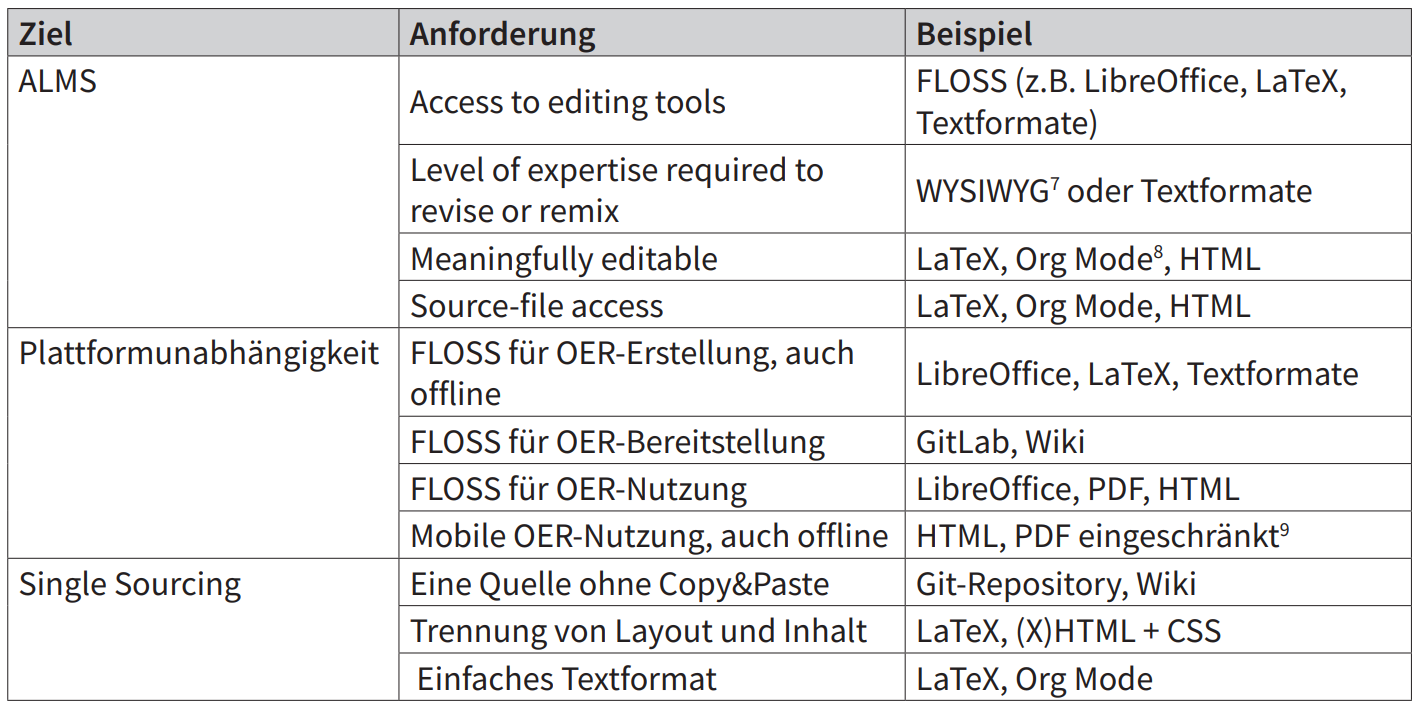
\includegraphics[width = 16cm]{alms_framework.png}
\caption{Anforderungen an OER-Software \cite{Lechtenborger.2019}}
\label{Anforderungen an OER-Software}

\end{center}
\end{figure}


Die zweite Anforderung des ALMS-Frameworks fordert eine möglichst geringe Expertise, die zur Nutzung der Software erforderlich ist. Hier sind Kundensegmente zu berücksichtigen, die eher eine geringere Affinität zu Computern aufweisen. Demnach ist die Benutzeroberfläche intuitiv zu gestalten und die Nutzung der Anwendung sollte auch ohne Programmierkenntnisse erfolgen können.

Die beiden letzten Kriterien des Frameworks sind eng miteinander verknüpft. Unter \glqq Meaningfully editable \grqq{} wird die Editierbarkeit der Materialien gefordert, während beim \glqq Source-file access \grqq{} dessen mögliche Verfügbarkeit verstanden wird. Sind die Quelldateien der Karteikarten nicht verfügbar, können die Karten folglich auch von keiner anderen Person bearbeitet werden. \\

Als Erweiterung zum ALMS-Frameworks wird die Plattformunabhängigkeit für die Erstellung, Bereitstellung und Nutzung der Materialien, wie auch eine freie Software gefordert. Die Nutzung der Materialien sollte möglichst auch ohne eine Internetverbindung und auch auf mobilen Endgeräten möglich sein. 
Eine weitere Anforderung, die zwar ebenfalls nicht mehr zum ALMS-Framework gehört, jedoch zur Wiederverwendbarkeit eine wichtige Rolle spielt, ist das Prinzip \glqq Single-Sourcing\grqq{}. Die Trennung von Layout und Inhalt erleichtert das Übertragen der Karteikarten auch in andere Programme, da hier nur der Inhalt berücksichtigt werden muss. Die vom Inhalt getrennten Layoutvorschriften sind flexibel austauschbar. Auch weitere Kopien des Materials sind durch die Einhaltung des Prinzips nicht erforderlich. Denn wie beispielsweise in der Versionsverwaltung Git soll aufbauend auf einer Quelle das Bearbeiten und Versionieren von Karteikarten möglich sein.


Konsequenzen aus den Anforderungen von OER sind demnach die Veröffentlichung eines Quellcodes und die Entwicklung einer webbasierten Anwendung. Des Weiteren sind immer eine einfache Handhabung und kollaborative Funktionen, wie das Teilen und Weiterverarbeiten zu berücksichtigen. Die Anwendung soll jedem frei zugänglich zur Verfügung stehen und soll auch offline genutzt werden können. Durch die Einhaltung des Single-Sourcings könnten die Materialien auch in andere Anwendungen importiert werden, sofern Bedarf dazu besteht.

%\glqq committed and modified \grqq{}

\subsection{Methoden für ein effektives Lernen}
Damit das Gelernte nicht nur im Kurzzeitgedächtnis verbleibt und eine Reduzierung von Lernschleifen erreicht wird, werden Lernmethoden benötigt, die eine Speicherung in das Langzeitgedächtnis fördern. Aus vorhandener Literatur wurden drei Lernmethoden ausgewählt, die im Rahmen dieser Seminararbeit umgesetzt und im nachfolgenden Abschnitt erläutert werden.

\subsubsection{Leitner-Algorithmus}
Der heute wohl bekannteste Algorithmus zum Lernen von Karteikarten wurde von Sebastian Leitner im Jahr 1972 vorgestellt \cite{SebastianLeitner.1972}. Bei diesem Vorgehen werden die Karteikarten im Laufe einer Lernsession, entsprechend des Lernergebnisses von einer Phase in eine anderen Phase verschoben. Zu Beginn liegen alle neuen Karten in der niedrigsten Phase. Wird eine Karte richtig beantwortet, darf diese in die nächstgelegene Phase verlagert werden, ansonsten ist diese um eine Phase zurückzusetzen. Die jeweiligen Phasen unterliegen verschiedenen Zeitintervallen, meist in Einheiten von Tagen, die mit fortschreitenden Phasen stets zunehmen. Befinden sich Karten in einer der höchsten Phasen, sollte diese im Langzeitgedächtnis verankert sein. Im  Laufe der Zeit wurden weitere Versionen dieses Algorithmus entwickelt, bei denen beispielsweise die Karteikarte direkt in die erste Phase zurückgesetzt wird, nachdem diese falsch beantwortet wurde.

\subsubsection{Microlearning}
Eine weitere Lernmethode, die sich auch auf das Lernen von Karteikarten anwenden lässt, nennt sich Microlearning \cite{Hug.2005}. Hier wird das erfolgreiche Lernen durch temporär kurzen Lerneinheiten unterstützt, die allerdings nur das wirklich relevante Wissen enthalten sollte. Nach dem Paper von Ilona Buchem und Henrike Hamelmann \cite{Buchem.2010} sollte eine Lerneinheit maximal 15 Minuten dauern. Da die Konzentrationsspanne eines Kindes zwischen 12 und 16 Jahren im Schnitt bei 30 Minuten und bei einem Erwachsenen im Schnitt bei 90 Minuten liegt, kann der Lernende innerhalb der Lerneinheit seine gesamte Konzentration einsetzen \cite{konzentrationsspanne}. Wissenseinheiten sollten in kleinen und unabhängigen Einheiten aufgeteilt werden, in denen jeweils nur ein Thema behandelt werden sollte. Nach Abschluss solch einer kurzen Lerneinheit bekommt der Lernende ein direktes Feedback, erhält somit eine positive Bestätigung und kann so seine Lernmotivation steigern.


\subsubsection{Spaced Learning}
Mit Wiederholungen (\glqq spaced repetition \grqq{}) der Lerneinheiten in bestimmten vorgeschriebenen Zeitintervallen, stellt das Spaced Learning eine Erweiterung zum Microlearning dar. Angelehnt wurde die Methode an die Vergessenskurve von Ebbinghaus aus 1880 und wurde erstmals theoretisch im Jahr 2005 von Douglas Fields eingeführt \cite{Fields.2005}. Zur Umsetzung des Spaced Learnings gibt es verschiedene Algorithmen, wie auf Basis von neuronalen Netzen \cite{BartoszDregerPiotrWozniak.1998} oder die Familie des SuperMemo-Algorithmus \cite{supermemo}. 


Die zugrunde liegende Theorie von Ebbinghaus sagt aus, dass nach 20 Minuten der Lernende nur noch 60{\%} des gelernten Wissens wiedergeben kann. Nach 60 Minuten liegt die Abrufmenge nur noch bei 45{\%}, nach 24 Stunden nur noch bei 34{\%} und nach 6 Tagen liegt die Abrufmenge lediglich bei 23{\%}. Von dem insgesamt gelernten Wissen bleiben lediglich nur 15{\%} dauerhaft gespeichert \cite{Liss.2020}. Um diesen Effekt zu vermeiden, sollten die kurzen, im besten Fall aufeinander aufbauenden Lerneinheiten in regelmäßigen Abständen wiederholt werden. \\

Eine Studie, die sich mit dem Vergleich zwischen Spaced-Learning und dem Massenlernen bei Honigbienen beschäftigt, fand heraus, beim Vergleich von Lernpausen von 30 Sekunden, 3 Minuten und 10 Minuten führten die Pausen von 10 Minuten zum besten Ergebnis \cite{Menzel.2001}. Diese konnten nach 30 Minuten zwar weniger Wissen abrufen, erreichten jedoch meist 100{\%} am dritten Kontrolltag, was auf eine Speicherung in das Langzeitgedächtnis hindeutet. \\

Diese Erkenntnisse, angewendet auf die Karteikarten-Anwendung führen, mit ausser Achtlassung bestehender Algorithmen, zum nachfolgenden Ergebnis. Eine Lerneinheit sollte aus einer Kategorie bestehen, kann aber auch bei Bedarf alle Karten in einer Kollektion berücksichtigen. Diese Lerneinheit hat eine maximale Dauer von 15 Minuten. Bei Beantwortung einer Frage wird ein Zeitstempel angelegt, der den Startzeitpunkt der nächsten Wiederholung festlegt. Nach Abschluss einer Lerneinheit kann, unabhängig von den Startzeiten der Karteikarten, die nächste Einheit frühstens nach 10 Minuten wieder gestartet werden. Ist diese Pause abgelaufen, sind die nächsten Karteikarten mit erreichen dessen Startzeit wieder aufrufbar.

%Eine andere Methode, wie sie in Anki eingesetzt wird ist die 

%Empfehlenswert sind 3 Einheiten zu einem Thema mit jeweils einer 10-minütigen Pause nach einer Einheit \cite{Kelley.2013b}. Diese Lernpausen können beispielsweise für unabhängige Zwischenspiele genutzt werden, um die Gedanken von dem Gelernten abzulenken. Ein weiterer Effekt dieser Lernmethode ist, wie auch beim Microlearning das regelmäßige und in kurzen Abständen auftretende Feedback, welches zu Erfolgsgefühlen führen und die Motivation steigern kann. 

%Weiterhin führen vielfältige Darstellungsformen, interaktive Elemente und ein Bezug in eigene Alltagserfahrungen und Alltagsgeschehen auch dazu, die Speicherung von Informationen in das Langzeitgedächtnis zu fördern. Im Rahmen der digitalen Verarbeitung können dazu vielfältige Methoden implementiert werden, die Abwechslung in die Einheiten bringen. Zum einen können mehrere Sinne angesprochen werden, wie mit einer Audioausgabe oder durch die Touchfunktion, wie auch mit verschiedenen Zwischenspielen. 



%http://super-memory.com/articles/theory.htm
%http://super-memory.com/english/algsm11.htm
%http://learnmem.cshlp.org/content/8/4/198.short


% Later research demonstrated two waves of transcription are required for LTM in honeybees: an early transcription wave (triggered during conditioning) and another starting several hours after learning (Lefer et al., 2012), as well as consolidation of LTM during sleep (Beyaert et al., 2012). 

\subsection{Berücksichtigung eigener Erfahrungen}
Nach mehrjähriger Erfahrung mit Karteikartenanwendungen kamen stets immer häufiger Änderungswünsche an der gerade genutzten Software auf. Diese Einblicke sind in dem Konzept der Anwendung berücksichtigt und werden nachfolgend kurz erläutert. \\

Eine Sortierung der Kurse nach definierten Prioritäten oder Fälligkeiten kann dabei helfen, die Konzentration auf relevante, anstelle von nebensächlichen Kursen zu richten.

Zur Verwaltung von obsoleten Kursen könnte eine Funktion zur Deaktivierung implementiert werden. Wahlweise kann dies auch durch den Export von Kursen auf lokale Datenspeicher geschehen, um mögliche Serverkapazitäten einzusparen und die Daten zusätzlich sichern zu können. \\

Auch bei der Erstellung von Karteikarten gibt es einige Anforderungen, die aus meiner Sicht einen hohen Stellenwert besitzen. Zum einen sollte die Erstellung einfach und zügig erfolgen. Zum Anderen wäre eine Festlegung der Relevanz von Karten sinnvoll oder die Festlegung von Prioritäten und Fälligkeitstermine für Kurse und Kategorien. 

Ein weiteres wichtiges Kriterium ist die Bearbeitungsmöglichkeit des Textes. Einige Anwendungen weisen hier schwere Mängel auf, die sich beispielsweise durch fehlende Hoch-, und Tiefstellungsmöglichkeiten bemerkbar machen. Da Karteikarten nicht mehr nur für das Lernen von Sprachen verwendet werden, sondern auch für mathematische oder chemische Kurse, ist eine Implementierung von Möglichkeiten zur Eingabe von Formeln notwendig. Viele Karteikarten-Anwendungen bieten nur die Möglichkeit diese Formeln als Bild zu speichern, was die Editierbarkeit jedoch einschränkt. Die Speicherung von Bildern ist eine weitere wichtige Anforderung, die hier erwähnt werden soll. Optimaler Weise wäre die Einbettung von Bildern im Textfluss, auch per einfacher copy {\&} paste-Funktion, anstelle eines Filedialogs. \\

Zusätzlich zu den vorgestellten Lernalgorithmen könnten noch weitere Methoden implementiert werden, wie Abfragen ausgerichtet nach Fälligkeiten. Hier könnten die Karten und dessen Anzahl mit Hilfe von Prognosen festgelegt werden. Eine weitere Methode wäre die eigene Zusammenstellung von Karten innerhalb einer anderen Lernsession, um diese gezielt auswendig lernen zu können. Diese willkürlichen oder aufeinander abgestimmten Karten werden dann so oft wiederholt, bis alle Karten richtig beantwortet wurden. Die letzte hier gewünschte Lernmethode ist die Abfrage der zehn schwierigsten Karten, nach Fehlerquote festgelegt. Im Idealfall sollte der Nutzer in der Lage sein zwischen verschiedenen Lernmethoden wechseln zu können. 

Eine Funktion, die in jeder Lernmethode angewendet werden kann, ist die Auswahl der Lernrichtung für bestimmte Kategorien oder Kurse. Somit können beispielsweise Vokabeln in beiden Richtungen gelernt oder Antworten den entsprechenden Fragen zugeordnet werden. \\

Um eine visuelle Bestätigung und Belohnung zu erhalten sind grundlegende Statistiken erforderlich. Zu einer der grundlegenden Funktionen zählt die Auflistung der Karten in den jeweiligen Phasen, sowie der Aktivitätsverlauf für den Anreiz einer lückenlosen Lernaktivität. Nach einer Lernsession sollte eine Erfolgsquote visualisiert werden, um die Motivation zu steigern. Zusätzlich zu den Statistiken zum vergangenen und aktuellen Verhalten bzw. dem Lernstand, sind Prognosen von fälligen Karten der nächsten Tage wünschenswert. \\

Für eine Individualisierung an eigene Bedürfnisse sind weitere verschiedenste Optionen notwendig. Beispielsweise mit inbegriffen ist die Festlegung der Anzahl von Karteikarten, die an einem Tag abgefragt werden, oder auch die Anzahl an neuen Karten, die täglich dazukommen können. Auch die Handhabung bei falsch beantworteter Frage könnte hier definiert werden, wie die Zurückstellung in die Anfangsphase oder nur die Zurückstellung in die nächst zurückliegende Phase. Alternativ zu den Zeitintervallen der Phasen, könnte auch eine Wahrscheinlichkeit implementiert werden, die das Auftreten der Karten innerhalb einer Lernsession definiert. Zur Unterstützung der individuellen Lerngeschwindigkeit könnte auch eine Bestimmung der Anzahl von Phasen behilflich sein. 

% Sicherheit


\section{Evaluation vorhandener Software}
Zur Auswertung der Konkurrenzangebote wurden 5 gängige Karteikarten-Anwendungen identifiziert. Mit in der Evaluation inbegriffen ist die gewählte Implementierungsgrundlage, auf der die hier entwickelte Software aufgebaut wird. In der nachfolgenden Abbildung sind alle herausgearbeiteten Anforderungen und dessen Erfüllungsart in den jeweiligen Software-Produkten aufgelistet. Für jedes dieser Produkte werden anschließend noch nennenswerte Eigenschaften erläutert, die nicht in Abbildung 2 vorhanden sind.

\begin{figure}[htbp]
\begin{center}
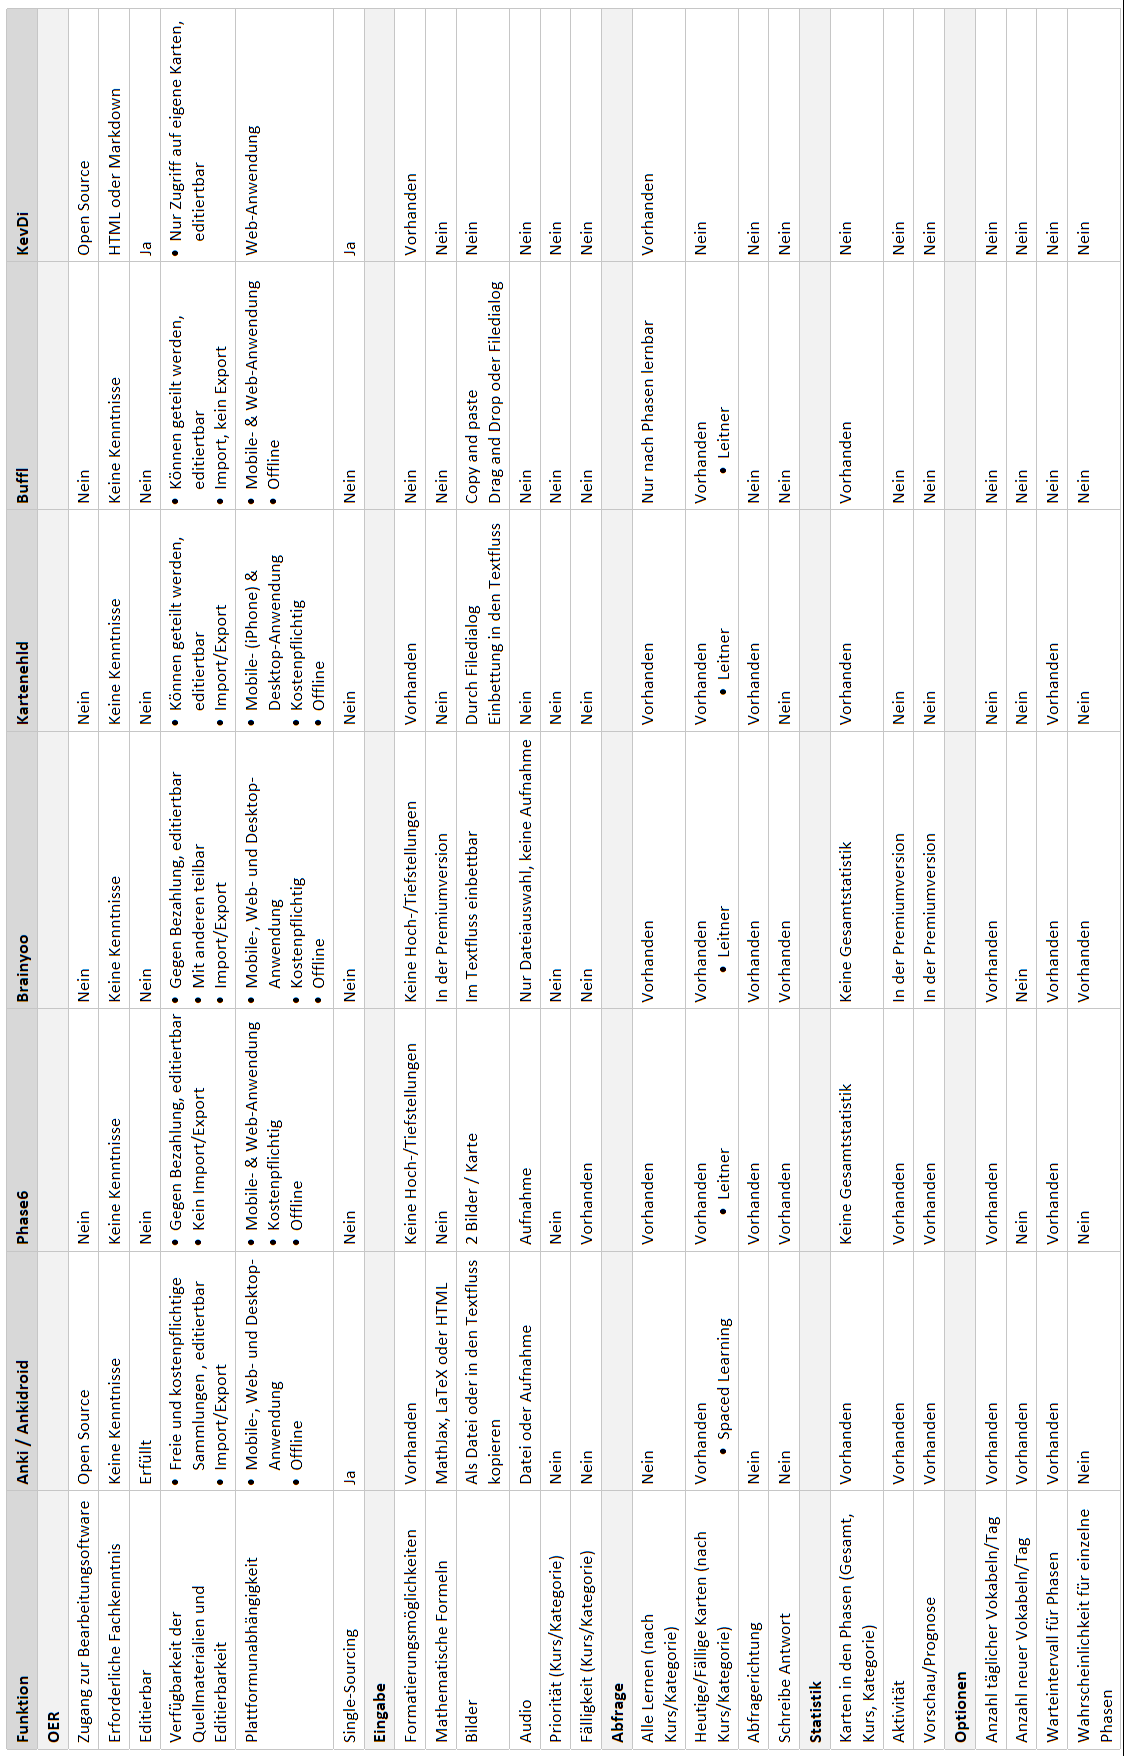
\includegraphics[width = 15cm, height=23cm]{evaluation.png}
\caption{Evaluation bekannter Karteikartenanwendungen}
\label{Evaluation bekannter Karteikartenanwendungen}

\end{center}
\end{figure}

\subsection{Anki und Ankidroid}
Die auf Open Source basierende Karteikarten-Applikation Anki \cite{ankiwebseite} \cite{ankidev} ist die funktionsstärkste Anwendung, die im Rahmen der Recherche gefunden wurde. Durch die Beliebtheit und der Möglichkeit einer gemeinschaftlichen Entwicklung arbeiten viele Entwickler an der fortlaufenden Verbesserung und Erweiterung. Erkenntlich wird dies beispielsweise bei der Eingabe von Karten. 
Eine Kartenseite kann in mehreren Sektionen aufgeteilt werden, die einen einheitlichen Aufbau vorschreiben. Im Beispiel von Vokabeln kann eine Karte in Wort, Bedeutung, einem Beispielsatz und einem Bild aufgeteilt werden. Weiterhin ist auch eine n-dimensionale Karte erstellbar, die nicht nur Frage und Antwort sondern beispielsweise auch eine Kartenseite mit einer Eselsbrücke enthält.  
Während der Eingabe können Bilder flexibel und zügig per copy {\&} paste in den Textverlauf eingefügt werden. Auch mathematische und chemische Formeln sind mit verschiedenen Methoden möglich. \\

Im Bezug von Lernmethoden ist Anki eine von wenigen Karteikarten-Anwendungen, die Spaced Learning implementiert hat. Innerhalb der Statistik wird auch die Gedächtnisleistung nach Tageszeit berechnet. Eine hervorzuhebende Einstellungsmöglichkeit ist die Vermeidung von ähnlichen Karten, die sonst am selben Tag gelernt werden würden. Zur besseren Orientierung über die Qualität der vorgefertigten Karteikarten-Sammlungen hat Anki ein einfaches Votesystem auf der Webseite aufgeführt, die jeweils nur die Anzahl der guten oder schlechten Bewertungen angibt. \\

Bezüglich des ALMS-Frameworks erfüllt die Anwendungen alle Anforderunge. Auch die Plattformunabhängigkeit wird durch AnkiDroid, der webbasierten-, sowie der Desktop-Version erfüllt und steht jedem frei und kostenlos zur Verfügung.
Jedoch wird die Anwendung den Anforderungen des Single-Sourcings nicht gerecht. Theoretisch können Exportdateien in einem GitHub-Repository bereitgestellt werden, jedoch wäre eine interne Versionsverwaltung im Bezug auf die Fachkenntnis wünschenswert. Innerhalb der Anwendungen können einfache Textformate verwendet werden. Diese werden intern nach HTML umgewandelt und können als einfache Textdateien oder als ein spezifisches Anki-Dateiformat exportiert werden. Verwendete Bilder sind abseits der Anki-Formate nicht speicherbar und können zur Weiterverarbeitung in anderen Programmen nicht verwendet werden. Auch fehlende Möglichkeiten zur Kommunikation innerhalb der Anwendung oder zur Bewertung von einzelnen Karten wird hier nicht unterstützt.
Ein weiterer Kritikpunkt ist das Design der Benutzeroberfläche der Desktop-Anwendung. Diese ist recht langweilig und trostlos gestaltet und folgt weniger modernen Designlayouts. 
Auch die Anwendung an sich ist unübersichtlich gestaltet und mach einen überladenen Eindruck. Die in den Anfängen befindliche webbasierte Version von Anki ist dahingegen Verbessert worden, beinhaltet jedoch noch nicht den vollen Funktionsumfang und eine noch eine unausgereifte Benutzeroberfläche. \\


\subsection{Phase6}
Um mit Phase6 \cite{phase6} sinnvoll Lernen zu können, benötigt der Benutzer eine kostenpflichtige Premiumversion. Ein weiterer Kritikpunkt ist, dass der Quellcode der Software, sowie die Quelldateien der Karteikarten nicht öffentlich zur Verfügung gestellt werden. Durch die fehlende Exportfunktion wird auch die Forderung des Single-Sourcings nicht erfüllt. Durch mangelnde Formatierungsmöglichkeiten, wie fehlende Hoch- und Tiefstellungsmöglichkeiten, ist die Editierbarkeit innerhalb der Anwendung zudem eingeschränkt.
Auch die Möglichkeit Kollektionen zu deaktivieren ist bei Phase6 nicht möglich. Somit bleibt dem Nutzer nur die Möglichkeit diese vollständig zu löschen oder dauerhaft in der Anwendung zu belassen, was nach einiger Zeit jedoch ziemlich unübersichtlich werden kann. Nennenswert bei Phase6 ist jedoch die Option, die Anzahl der Phasen individuell bestimmen zu können, sowie die Verfügbarkeit auf mobile Endgeräten.\\


\subsection{BRAINYOO}
Wie auch bei Phase6 ist auch die Anwendung BRAINYOO \cite{brainyoo} für den Nutzer kostenpflichtig. Für Unternehmen und Schulen besteht allerdings die Möglichkeit die Software auf Anfrage für den internen Einsatz auf eigene Server zu hosten. Somit können sie eine gemeinschaftliche Umgebung zum Lernen von Karteikarten für unterschiedlichste Zwecke bereitstellen und Statistiken über den Lernfortschritt der Teilnehmer einsehen. Zum diesem Zweck können für Kollektion auch Lerngruppen erstellt werden. Eine gemeinschaftliche Bearbeitung ist allerdings nicht vorgesehen. Jedoch können die Karteikarten in einem XML-Dateiformat exportiert werden. Auch BRAINYOO erfüllt nicht alle technischen Anforderungen an OER.
Außergewöhnliche Funktionen sind jedoch der Power-Lernmodus, indem anstelle von Tage, eine Wahrscheinlichkeit angegeben werden kann, mit der Karten aus den Phasen ausgewählt werden. Für jede Karte könnte der Nutzer neben Frage und Antwort auch eine Eselsbrücke angegeben, die ihm beim Lernen helfen kann.

\subsection{Kartenheld}
Die Anwendung Kartenheld \cite{kartenheld} ist eine ziemlich einfach gehaltene Software, die von Rico Gundermann entwickelt wurde und dem von Microsoft vertrautem Design folgt. Nach einer kostenlosen Testversion ist der Benutzer dazu verpflichtet sich eine Lizenz zu kaufen, was auf Grund der fehlenden Funktionen nicht empfehlenswert ist. Ein Erstellen neuer Karten ist nach Ablauf der Testversion nicht mehr möglich, da diese nun nur noch im schreibgeschützen Modus zur Verfügung steht. Der Quellcode ist ebenfalls nicht für die Öffentlichkeit verfügbar. In Kartenheld ist es dem Benutzer nicht möglich Kategorien für einzelne Kurse zu erstellen, Statistiken einzusehen oder Einstellungen, abgesehen von den Zeitintervallen für einzelne Phasen zu treffen. Als einzige Statistik ist hier die Anzahl der Karteikarten in den einzelnen Phasen zu nennen. Da auch die Dateien nur in einem spezifischen .flashcard-Dateiformat speicherbar sind, erfüllt auch diese Anwendung nicht alle Anforderungen AN OER-Software.
Positiv für Kartenheld ist jedoch die Möglichkeit Multiple Choice Aufgaben zu erstellen, die eine Abwechslung zum traditionellen Kartendesign darstellen. Auch die mögliche Abfrage nach schwierigen Karteikarten ist hier als nützliche Funktion zu nennen. Eine weitere Funktion ist die Auswahl der Phasen für eine Lernabfrage, auch wenn diese noch nicht für eine Abfrage fällig ist. \\


\subsection{Buffl}
Buffl \cite{buffl} ist eine funktional schlicht gehaltene Anwendung, die trotz dessen nicht intuitiv aufgebaut ist. Der Quellcode ist auch hier wieder nicht öffentlich verfügbar, doch für den Benutzer ist die Anwendung kostenlos. Die Kartenmodelle in Buffl sind mit verschiedenen Kartenmodellen eingeschränkt und es sind nur Kombinationen von Text, Listenpunkte und Bild möglich. Die Kurse können mit anderen Lernenden per Link, E-Mail Adresse oder Benutzername zum Lernen geteilt werden. Auch ist ein Import aus dem eigenen System möglich, allerdings ist eine Exportfunktion bisher nicht vorhanden und der Nutzer kann auf die Quelldateien nicht zugreifen. \


\subsection{KevDi als Grundlage für die Entwicklung}
Die webbasierte Anwendung von KevDi \cite{kevdi}, die auf GitHub verfügbar ist, weist einen recht spärlichen Funktionsumfang auf. Die Benutzeroberfläche ist schlicht gehalten und macht einen benutzerfreundlichen Eindruck. Der Benutzer hat lediglich die Möglichkeit auf eigene Kurse und Karteikarten zuzugreifen. Für die Eingabe und der Formatierung von Texten ist entweder die Sprache Markdown oder HTML notwendig. In der untersuchten Version von KevDi ist es bisher nicht möglich, Kurse zu bearbeiten oder weitere Kategorien für Kurse zu erstellen. Auch Bilder, mathematische Formeln oder das Abspielen von Audiodateien ist bisher nicht möglich. Als Lernmethode wurde weder das Leitner, noch das Spaced Learning implementiert. Hier hat der Nutzer nur die Wahl alle Karten eines Kurses zu durchlaufen bis alle Karten einmal beantwortet wurden. Im den nächsten Durchläufen werden alle falsch beantworteten Fragen so oft wiederholt, bis alle Fragen richtig beantwortet wurden. In dieser Version sind bisher noch keine Einstellungsmöglichkeiten, Statistiken, Export- oder kollaborative Funktionen vorhanden. \\

Die Anwendung wurde trotz der mangelnden Funktionen als Entwicklungsgrundlage ausgewählt. Der Grund für diese Entscheidung ist unter anderem die schon vorhandene Benutzeroberfläche, die mit Hilfe der Python-Bibliothek Flask und den Designelementen von Bootstrap erstellt wurde. Zum anderen bot die Anwendung einen leichten Einstieg in den Quellcode und die Möglichkeit die Applikation von Grund auf aufzubauen, ohne die Funktionen zur Benutzerauthentifizierung zu implementieren. Auch die Anbindung an einen Web- und E-Mail Server sind schon vorhanden und so konnte sich auf die Implementierung der wesentlichen Funktionen konzentriert werden. \\



\section{Dokumentation der webbasierten Anwendung Kicards}
Auf Grundlage der vorher ermittelten Anforderungen und Funktionen, ist das Ziel dieser Seminararbeit eine webbasierte und effiziente Anwendung zu entwerfen \cite{kicards}, die den Anforderungen an OER-Software gerecht wird. Zu diesem Zweck werden zunächst alle benötigten Funktionen aufgelistet, um in einem nächsten Schritt eine Datenbank zu modellieren.

\subsection{Funktionsübersicht}
In der nachfolgenden Abbildung 3 werden alle zu implementierenden Funktionen in \emph{must-, could-, und should-have}-Kategorien eingeteilt, um eine Priorisierung und einen Laufplan für die Entwicklung zu erhalten. \\

\begin{figure}[htbp]
\begin{center}
\includegraphics[width = 15cm, height=23cm]{must3.png}
\caption{Priorisierte Funktionen der Anwendung Kicards}
\label{Must-,Should-, Could-Have der Anwendung Kicards}

\end{center}
\end{figure}

Zunächst sind die Anforderungen an OER-Software zu finden, die alle in die \emph{must-have}-Kategorie eingeordnet wurden. 
Die Freiheit der Bearbeitungssoftware und dessen Zugriff wird durch die Bereitstellung auf GitHub gewährleistet \cite{kicards}. Auch die Quellmaterialien könnten hier zur Verfügung gestellt werden. 
Weiterhin wird eine Reduzierung der Fachkenntnis, durch die Anzeige der wichtigsten Syntax für die Formatierung des Textes, während der Erstellung und Bearbeitung von Karteikarten erreicht. Die hier genutzten Sprachen Markdown und HTML tragen zudem dazu bei, die Anforderung der Editierbarkeit zu erfüllen.
Zur Erfüllung der Anforderung \glqq Source-file access\grqq{} werden Import- und Exportfunktionen implementiert, die auf eine Trennung von Layout und Inhalt abzielen und in einfachen Textdateien aufrufbar sind. 
Neben der Trennung von Layout und Inhalt ist eine weitere Forderung des Single-Sourcings mit nur einer Quelldatei zu arbeiten, ohne die Erzeugung unnötiger Kopien. Dies soll durch ein internes Versionskontrollsystem erreicht werden, welches auch die benötigte Fachkenntnis weiter reduzieren soll. 
Die Plattformunabhängigkeit wird zunächst durch eine webbasierte Anwendung erreicht. In der späteren Entwicklung soll Kicards auch offline und auf mobilen Endgeräten zur Verfügung stehen. \\

Weitere allgemeine Funktionen sind zum einen ein ansprechendes Design, welches dem Nutzer zum Lernen motiviert oder eine Übersicht der abzuarbeitende Kursen, ggfs. nach Prioritäten oder Fälligkeiten sortiert. Weiterhin sollten während der Eingabe mathematischer Formeln, Bilder und Audiodateien verarbeitet werden können. \\

Statistiken können den Nutzern dabei helfen, die Motivation zu steigern. Übersichten über Karten in den verschiedenen Phasen oder dem Lernfortschritt nach einer Lernsession, sind Beispiele für solche Statistiken. Weitere Beispiele sind die Benutzeraktivität oder Prognosen über zukünftig anfallende Karten. Die Gedächtnisleistung nach Tageszeit, wie in Anki implementiert, ist eine sehr nützliche Funktion, um sein Lernverhalten dementsprechend anzupassen. Sie erhält hier jedoch zunächst eine niedrigere Relevanz. \\

Notwendige Einstellungsmöglichkeiten wurden nicht identifiziert. Optionen, wie die Anzahl der täglichen Vokabeln oder der neuen Vokabeln pro Tag könnten bereitgestellt werden, sind jedoch nicht zwingend erforderlich. Weitere Möglichkeiten betreffen die Handhabung der Phasenzurücksetzung oder das Warteintervall für einzelne Phasen. Zusätzliche Optionen, die allerdings in die \emph{could-have}-Kategorie fallen, sind die Vermeidung verwandte Karten am selben Tag zu lernen oder Wahrscheinlichkeiten für Phasen anzugeben. 

\subsubsection{Lernmethoden}
Die Leitner-Methode wird zunächst mit einer festen Anzahl von 8 Phasen implementiert. In der ersten Phase 0 werden zunächst neu erstellte Karten abgespeichert, die bisher noch nicht gelernt wurden. Die darauffolgenden Phasen sind mit Wartezeiten in Tagen oder einer Wahrscheinlichkeit ausgestattet. Diese legen fest, wann eine Karte wiederholt. Nach richtiger Beantwortung einer Frage in der Lernsession "Leitner" wird das nächste Abfragedatum, entsprechend der neuen Phase aktualisiert. Während bei einer falschen Beantworten das nächste Abfragedatum unberührt bleibt. In beiden Fällen wird jedoch das letzte Abfragedatum aktualisiert.

Beim Spaced-Learning Algorithmus werden die Fragen nicht mit Richtig oder Falsch beantwortet, sondern durch Einteilung \emph{nochmal}(0 Sek), \emph{schwer} (10 Min), \emph{mittel}(60 Minuten), \emph{leicht}(6 Tage) und \emph{ganz leicht}(30 Tage) eingeordnet. Auch hier wird jeweils dementsprechend das nächste Abfragedatum verändert. 
Eine Lernsession hat bei dieser Methode eine Gesamtdauer von 15 Minuten. Nach Ablauf einer Einheit ist eine neue Session erst nach einer 10 minütigen Pause wieder startbar. Dadurch soll die Aufnahmefähigkeit, unter anderem durch Anwendung des Mircolearnings gesteigert werden. \\

Beim Start der Lernmethode \glqq{}schlechtesten Karten\grqq{} werden aus der ausgewählten Kollektion zunächst alle Karten ermittelt. Von diesen ermittelten Karten werden jeweils die 10 schlechtesten Fehlerquoten identifiziert und zur Lernsession hinzugefügt. Diese werden dann im weiteren Verlauf solange wiederholt, bis alle Karten richtig beantwortet wurden. \\

Die Lernmethode \glqq{}nach Fälligkeit\grqq{} ist etwas aufwändiger zu Implementieren. Hierzu ist eine Prognose erforderlich, die ermittelt, wie viele Karten durchschnittlich im Laufe eines Tages gelernt werden müssen um den Termin einzuhalten. Hierzu könnten Statistiken über die jeweilige Lerngeschwindigkeit oder auch Metadaten über die aktuelle Kollektion genutzt werden. \\

Für die nächste Lernmethode muss bei Erstellung oder Bearbeitung von Karten eine Relevanz von 0 (nicht wichtig) bis 5 (sehr wichtig) angegeben werden. Beim Start einer Abfrage kann der Nutzer festlegen, welchen Relevanzgrad er gerade lernen möchte. \\

Die Kartenauswahl für das intensive Lernen kann in jeder Abfrage mit dem Button \glqq für später merken\grqq{} ausgewählt werden. Kehrt der Nutzer zur Übersicht der Kollektion zurück, kann dieser eine intensive Session mit den ausgewählten Karten starten. Nach einem Durchlauf der Lernsession wird diese dann so oft wiederholt, bis alle Karten in einer Session richtig beantwortet wurden.


\subsubsection{Kollaboratives Lernen und Bearbeiten}
Um das kollaborative Arbeiten zu Unterstützen sind verschiedenste Funktionen notwendig. Zunächst müssen Kollektionen auch als öffentliche Kurse zur Verfügung gestellt werden können. Um einer Kollektion dann als Nutzer zu folgen, kann er sich hierzu als Follower eintragen. Neben dem Lernen bekommt ein Follower das Recht, dem Ersteller einer Karte einen Vorschlag zur Verbesserung einzureichen, sowie diesbezüglich weiterhin mit dem Ersteller zu kommunizieren. Andere Teilnehmer einer Kollektion können diesen Vorschlag ebenfalls einsehen, wenn diese dazu eine Schaltfläche zur Einblendung betätigen. Auch kann er weitere Karten zur Kollektion, durch eine direkte Erstellung oder einem Import hinzufügen. Ihm sollte zudem die Möglichkeit eingerichtet werden, öffentliche Kollektionen auf lokale Systeme zu speichern, um diese auch offline Nutzen, eigene Versionen zu erstellen oder die Dateien in anderen Programmen öffnen zu können. \\

Um schlechte Karten aussortieren zu können, wird ein Votesystem für jede Karteikarte implementiert. So können Karten, auch ohne eine Zustimmung des Erstellers gelöscht werden, sobald ein gewisser Prozentsatz dafür stimmt. Um die Anzahl der Follower eines Kurses nicht durch langfristig inaktive Nutzern zu verfälschen, werden diese nach einer gewissen Zeit aus der Liste der Follower entfernt. 

\subsection{Datenbankmodellierung}
Der nächste Schritt, nach Festlegung der geforderten Funktionen besteht in der Modellierung der Datenbank. Hier wird im ersten Schritt das Datenbankmodell in Abbildung 4 skizziert und anschließend die Zusammenhänge und Abhängigkeiten erläutert.  

\begin{figure}[h]
 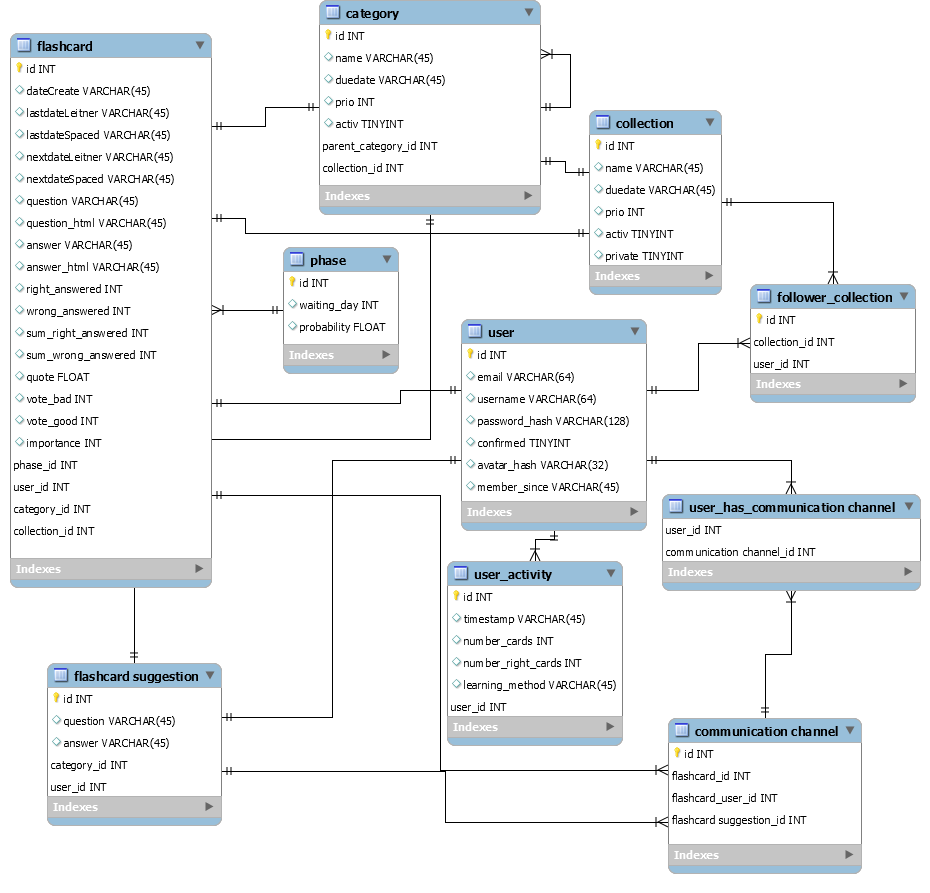
\includegraphics[width = 15cm]{databasemodel.png}
 \caption{Datenbankmodel von Kicards}
 \label{fig:datenbankmodel}
\end{figure}

% \glqq Text \grqq{}

Im Mittelpunkt des Datenbankmodells steht die Tabelle Karteikarte (\emph{flashcard}). Eine Karteikarte hat Attribute, wie die Phase (\emph{phasen{\_}id}), das Erstellungsdatum (\emph{dateBeginn}), jeweils ein Datum für die letzte Abfrage der Leitner-Methode (\emph{lastdateLeitner}) und ein Datum für den Spaced-Algorithmus (\emph{lastdateSpaced}), ebenso wie für die nächsten Abfragen (\emph{nextdateLeitner}, \emph{nextdateSpaced}). Für die Aufnahme der Frage und Antwort sind die Felder \emph{question} und \emph{answer} vorgesehen, die mit Hilfe einer Umwandlung in HTML auch die Felder \emph{question{\_}html} und \emph{answer{\_}html} belegen. Für die Ermittlung der Fehlerquote werden die Felder \emph{right{\_}answered} and \emph{wrong{\_}answered}, sowie die Summen \emph{sum{\_}right{\_}answered} and \emph{sum{\_}wrong{\_}answered} benötigt. Die Fehlerquote wird nach Aktualisierung in dem Feld \emph{quote} gespeichert. Um die Umsetzung des Votesystems für einzelne Karteikarten implementieren zu können, werden die Felder \emph{vote{\_}bad} und \emph{vote{\_}good} benötigt. Jede Karteikarte hat einen Ersteller, der in dem Attribut \emph{user{\_}id} gespeichert wird und eine Referenz zur Tabelle User enthält. Als letztes Attribut wird hier die Relevanz (\emph{importance}) gespeichert. Jede Karteikarte gehört zu genau einer Kategorie und Kollektion, die jeweils durch die Felder \emph{collection{\_}id} und \emph{category{\_}id} modelliert wird.

In der Tabelle Kategorie (\emph{category}) befinden sich die Felder \emph{name} der den Namen der Kategorie enthält und das Feld \emph{duedate} für den Fälligkeitstermin. Zudem kann der Kategorie eine Priorität (\emph{prio}) zugeordnet werden. Um zu Bestimmen ob eine Kategorie gerade aktiv ist, d.h. zum Lernen bereitsteht, kann durch das Feld \emph{activ} ermittelt werden. Zu jeder Kategorie gehört eine Kollektion, die durch das Feld \emph{collection{\_}id} dargestellt wird. Jede Kategorie kann jeweils mehrere Unterkategorien enthalten, die durch das Feld \emph{parent{\_}category} dargestellt wird.

Die Tabelle der Kollektionen enthält ein Feld für den jeweiligen Namen (\emph{name}), ein Fälligkeitstermin (\emph{duedate}), eine Priorität (\emph{prio}) und auch ein Feld, um zu bestimmen, ob eine Kategorie aktiv ist oder deaktiviert wurde. Zusätzlich gibt es ein Feld, um zu Bestimmen ob eine Kategorie nur privat ist, oder für die Öffentlichkeit freigegeben wurde. 

Eine Kollektion kann von mehreren Benutzern verfolgt werden. Hierzu gibt es eine Tabelle \emph{follows{\_}collection}, die eine n:n-Beziehung zwischen Benutzer und Kollektionen darstellt. Zu diesem Zweck wird jeweils eine \emph{collection{\_}id} und eine \emph{user{\_}id} gespeichert. 

In der Tabelle Benutzer werden die E-Mail Adresse (\emph{email}), der Benutzername (\emph{username}), das Passwort in Form eines Passwort-Hashes (\emph{password{\_}hash}) und ein boolisches Feld gespeichert, in dem festgelegt wird, ob das Benutzerkonto bestätigt wurde. Zur Speicherung eines Benutzerfotos wird ein \emph{Avatar{\_}Hash} gespeichert. Als letztes Attribut wird hier das Erstellungsdatum des Benutzerkontos angegeben (\emph{member{\_}since}).

Die letzte Tabelle stellt die Aktivitäten des Benutzers dar. Diese wird hauptsächlich für die Ermittlung der Aktivitätsstatistiken verwendet. Hierzu wird der jeweilige Benutzer (\emph{user{\_}id}), ein Zeitstempel (\emph{timestamp}), die Anzahl der in einer Lernsession richtig beantworteten Karten, sowie die Gesamtzahl der Karten, die in dieser Session behandelt wurde. Als letztes Attribut wird noch die Lernmethode (\emph{learning{\_}method}) erfasst, um die Aktivität nach Methode filtern zu können.


\section{Aktueller Entwicklungsstand und Ausblick}
Im Rahmen dieser Seminararbeit konnte erst ein Teil des Funktionsumfang der Anwendung implementiert werden und wird innerhalb der Abbildung 3 dokumentiert. Die Arbeit stellt jedoch ein Konzept für Karteikarten bereit, auf dem in weiteren Entwicklung aufgebaut werden kann. Zwar wurde noch nicht alle Funktionen umgesetzt, jedoch konnten die meisten \emph{must-have}-Anforderungen und viele \emph{should-have}-Anforderungen erfüllt werden. 

Die Kriterien an OER-Software wurden bisher größtenteils erfüllt. In weiteren Entwicklungsschritten soll zunächst eine mobile Anwendung implementiert werden, die auch einen offline Nutzung der Karteikarten zulassen soll. Eine wichtige Funktionen einer mobilen Anwendung ist die Unterdrückung von Benachrichtigung, um den Lernfluss nicht zu unterbrechen.

Nach Fertigstellung aller grundlegenden Funktionen, die zunächst nur eine alleinige Nutzung ermöglichen sollen, können weitere Funktionen zur Erfüllung der OER-Kriterien entwickelt werden. 

Dies kann die Vorbereitung auf eine kollaborative Plattform sein. Hierzu soll zunächst das Votesystem für einzelne Karten erstellt. Anschließend Kommunikationsmöglichkeiten innerhalb einer Kollektion und ein Vorschlagsystem, um die Zusammenarbeit zu ermöglichen.\\

Auch die bisher noch nicht implementierte Lernmethode kann in einer späteren Entwicklung noch hinzugefügt werden. Das Lernen zu einem bestimmten Fälligkeitstermin benötigt verschiedene Statistiken, die hier noch erst erstellt werden müssten. Verbesserungen könnten sich auch durch weitere Untersuchung von Spaced-Learning Algorithmen ergeben, um die Lerneffizienz weiterhin zu steigern.

Für eine Erweiterung der Nutzergruppe kann die Anwendung noch internationalisiert werden. Hierzu kann beispielsweise eine Tabelle erstellt werden, in der alle Benachrichtigungen und  Beschriftungen in verschiedene Sprachen übersetzt werden. Mit einer Option zur Sprachauswahl in den Einstellung können dann alle Daten dementsprechend angepasst werden.

Nicht zuletzt sollten noch Sicherheitsaspekte und Pflichten aus dem Datenschutz berücksichtigt werden. Gefahren, wie SQL-Injektions werden zwar durch die wtf-Forms von Flask verhindert, jedoch könnten es andere Sicherheitslücken geben, die vorher geprüft werden sollten. \\

Kicards kann dazu beitragen die Hürden zur Bildung zu verringern. Sie soll sich dank des ausgearbeiteten Konzepts zu einer kollaborative Plattform entwickelt, die frei für jeden zugänglich ist und effiziente Lernmethoden anbietet, mit der Lerneinheiten langfristig in Erinnerung bleiben

% The following is for the Emacs users out there... :-)
%%% Local Variables:
%%% mode: latex
%%% TeX-master: "guide2seminars"
%%% eval: (ispell-change-dictionary "en")
%%% End:
